\documentclass{article}
\usepackage{graphicx} % Required for inserting images
\usepackage{url}      % Useful for formatting URLs in bibtex
\title{Structured Hints for Sample-Efficient Lean Theorem Proving}
\author{Zac Burton \\ Massachusetts Institute of Technology}
\date{\today}

\begin{document}

\maketitle

\begin{abstract}
State-of-the-art neural theorem provers like DeepSeek-Prover-V1.5 combine large language models with reinforcement learning, achieving impressive results through sophisticated training. We ask: do these highly-trained models still benefit from simple structural guidance at inference time? We evaluate a lightweight intervention---a fixed prompt schedule over 15 common tactic skeletons---on the miniF2F benchmark. This simple approach yields 21.7\% pass@16 compared to 15.2\% for standard sampling from the same model, a 43\% relative improvement using the same number of samples ($k=16$) and same maximum generation length (1024 tokens). Our results suggest that even capable RL-trained provers underutilize structural priors available in the tactic language, and that simple inference-time guidance remains a cheap, complementary boost.
\end{abstract}

\section{Introduction}

Recent advances in neural theorem proving have demonstrated remarkable success by combining Large Language Models (LLMs) with formal verification environments like Lean. Systems leveraging reinforcement learning (RL) and massive tree searches have achieved strong results on formal proof benchmarks \cite{xin2024deepseek, chen2025seed, trinh2024solving}. The prevailing paradigm often assumes that with sufficient RL training and inference-time compute, models will implicitly internalize the necessary structural and tactic-level priors required for formal proofs.

However, despite these capabilities, neural provers remain surprisingly brittle. Even RL-trained models frequently fail due to low-level structural errors—generating invalid syntax, hallucinating identifiers, or getting ``lost" in the proof state space—rather than a lack of mathematical insight. This disconnect raises a critical question for resource-constrained settings: \textit{Has RL actually solved the structural problem, or can lightweight, fixed-schedule guidance still yield significant gains?}

In this work, we investigate whether enforcing structural priors at inference time improves performance under the same inference budget. Unlike recent approaches that rely on expensive stochastic search or massive sampling (e.g., $k=1024$), we propose a lightweight \textbf{Intermediate Representation (IR)} with a fixed prompt schedule. By guiding the model with structural skeletons, we probe the behavioral limits of current RL-trained provers.

Our results on the \texttt{miniF2F} benchmark show that this simple structural guidance yields a \textbf{43\% relative improvement} over the baseline (15.16\% $\to$ 21.72\%) under a fixed, low-inference budget ($k=16$). Our paired analysis shows strong asymmetry (19 wins vs.\ 3 losses), indicating that tactic skeletons provide a robust boost rather than merely trading off between problem types.

\subsection{Contributions}
Our primary contributions are as follows:
\begin{itemize}
    \item We introduce a Lean-aware Intermediate Representation (IR) with a fixed prompt schedule that provides structural guidance at inference time.
    \item We demonstrate that this lightweight intervention significantly outperforms standard sampling on \texttt{miniF2F} under identical inference budgets ($k=16$, 1024 tokens).
    \item We provide a failure-mode analysis showing that error distributions are similar between methods; gains appear to come from a higher hit-rate on successful completions rather than systematic avoidance of particular error types.
\end{itemize}

\section{Related Work}

\paragraph{Neural Theorem Proving}
The integration of Language Models with formal proof assistants has evolved rapidly. Early systems like GPT-f \cite{polu2020generative} and PACT \cite{han2022proof} demonstrated that transformers could generate tactic scripts. More recent efforts, such as \textbf{LeanDojo} and its associated \textbf{ReProver} model \cite{yang2023leandojo}, introduced retrieval-augmented generation to handle the vast library of Lean premises. The current state-of-the-art is dominated by models trained with massive Reinforcement Learning (RL) pipelines, notably \textbf{DeepSeek-Prover-V1.5} \cite{xin2024deepseek} for Lean tactic generation and \textbf{AlphaGeometry} \cite{trinh2024solving} for geometry-specific formal reasoning, which rely on iterative self-improvement and synthetic data generation to achieve strong performance on formal benchmarks.

\paragraph{Neuro-Symbolic Reasoning}
Recent work has moved towards hybrid systems that interleave natural language reasoning with formal verification. \textbf{Aristotle} \cite{achim2025aristotle} achieved state-of-the-art results on IMO problems by generating and formalizing \textit{semantic lemmas} (intermediate mathematical statements) to bridge the gap between informal reasoning and formal proof. 

Our work targets a complementary, lower-level efficiency constraint. Rather than generating new mathematical lemmas (which requires heavy reasoning), we focus on \textit{syntactic skeletons}—enforcing valid tactic structures (e.g., \texttt{induction}, \texttt{cases}) at the start of generation, serving as a   \textit{hint} for the LLM's approach to the problem. We demonstrate that this lightweight structural guidance captures significant performance gains in resource-constrained environments where full lemma synthesis is too costly.


\section{Method}

To evaluate the impact of structural guidance under strict inference constraints, we introduce an Intermediate Representation (IR) with a fixed prompt schedule. Unlike standard autoregressive generation which conditions solely on the theorem statement, our approach conditions the model on a structural tuple that explicitly separates proof planning from tactic execution.

\subsection{Structured Intermediate Representation}
Formally, let $\mathcal{T}$ be the space of theorem statements in Lean, and $\mathcal{P}$ be the space of valid tactic sequences. We define a \textbf{Structured Query} $q$ as a tuple:
\begin{equation}
    q = (x, s)
\end{equation}
where:
\begin{itemize}
    \item $x \in \mathcal{T}$ is the formal theorem statement (the goal).
    \item $s \in \mathcal{S}$ is a \textit{tactic skeleton} (a prefix of tactics representing the high-level proof strategy, e.g., \texttt{simp}, \texttt{intro}, \texttt{constructor}).
\end{itemize}

The generation process is modeled as $P_{\theta}(y \mid x, s)$, where the model $\theta$ is constrained to complete the proof $y$ given the enforced structural start $s$. This effectively ``locks" the model into a specific proof strategy before inference begins, reducing the search space of valid next tokens.

\subsection{Fixed Prompt Schedule}
Instead of relying on stochastic temperature sampling alone, we enforce diversity through a fixed prompt schedule. For a given theorem $x$, we generate a set of $k=16$ distinct queries $Q_x = \{q_1, \dots, q_{16}\}$ by iterating over a fixed set of 15 tactic skeletons (including the empty skeleton; full list in Appendix~\ref{app:prompts}). The 16th attempt reuses the empty skeleton, yielding one duplicate in the schedule.\footnote{Our implementation also supports optional natural-language goal hints; for this paper we set all hints to $\emptyset$ except attempt 16, which includes a generic hint. Ablations isolating skeleton vs.\ hint contributions are left for future work.}

This schedule ensures that the model attempts a diverse range of proof strategies regardless of the model's internal probability distribution, which might otherwise collapse to a single, incorrect mode. Note that while the \textit{prompt schedule} is fixed, the model still samples stochastically (temperature $= 0.6$) to generate the proof completion.

\subsection{Experimental Setup \& Constraints}
\label{sec:constraints}
To strictly evaluate the model's structural efficiency without the confounding factor of massive search, we enforce strict computational constraints on all evaluations. Specifically, we limit generation to a maximum of \textbf{1024 tokens} and restrict sampling to $k=16$ attempts per theorem.

While recent benchmarks often utilize significantly larger budgets (e.g., $k=1024$, extended context windows), these approaches are computationally prohibitive for many practical applications. Our experimental design explicitly targets this resource-constrained regime to evaluate whether structural guidance can recover performance lost to limited compute. As such, our baseline results reflect this strict cutoff and should be interpreted as a \textit{low-latency performance floor}, rather than a ceiling of model capability.

\subsection{Evaluation Protocol}
\label{sec:evaluation}
We evaluate on \texttt{miniF2F-test} (Lean 4 split; 244 theorems) using DeepSeek-Prover-V1.5-RL\footnote{\texttt{deepseek-ai/DeepSeek-Prover-V1.5-RL} from HuggingFace} in completion-style prompting. For each theorem, we run up to $k=16$ attempts with a maximum of 1024 generated tokens per attempt under fixed decoding parameters (temperature $= 0.6$, top-$p = 0.95$; see Appendix~\ref{app:prompts} for the full prompt template). Each attempt is assembled into a Lean 4 file containing \texttt{import Mathlib} followed by the full benchmark theorem statement and \texttt{:= by} with the generated tactics. We compile using \texttt{lake env lean --json} inside a pinned Mathlib environment (Appendix~\ref{app:env}) with a per-attempt timeout of 60 seconds. A theorem is counted as solved if and only if Lean returns exit code 0; any output containing \texttt{sorry} is treated as failure.


\section{Results}

We evaluate the effectiveness of our approach on the \texttt{miniF2F-test} benchmark (Lean split), consisting of 244 formal theorems. We compare our Structured Intermediate Representation (IR) against the unguided Baseline under identical inference constraints ($k=16$, max\_tokens=1024).

\subsection{Main Performance}
Table \ref{tab:main_results} summarizes the pass rates. Our structured approach solves 53 theorems (21.72\%), compared to 37 theorems (15.16\%) for the baseline. This represents a net absolute gain of 6.56 percentage points and a \textbf{relative improvement of 43.2\%}.

\begin{table}[h]
    \centering
    \begin{tabular}{lccc}
        \hline
        \textbf{Method} & \textbf{Solved (N)} & \textbf{Pass@16 (\%)} & \textbf{Relative Gain} \\
        \hline
        Baseline (Unguided) & 37 / 244 & 15.16\% & - \\
        \textbf{Structured IR (Ours)} & \textbf{53 / 244} & \textbf{21.72\%} & \textbf{+43.2\%} \\
        \hline
    \end{tabular}
    \caption{Performance comparison on miniF2F-test. Both methods use DeepSeek-Prover-V1.5-RL with $k=16$ samples and a strict 1024-token limit.}
    \label{tab:main_results}
\end{table}

\subsection{Paired Analysis \& Overlap}
To understand whether our method simply solves a different subset of problems or strictly improves upon the baseline, we conducted a paired analysis of solved theorems (Figure \ref{fig:venn_breakdown}).
\begin{figure}
    \centering
    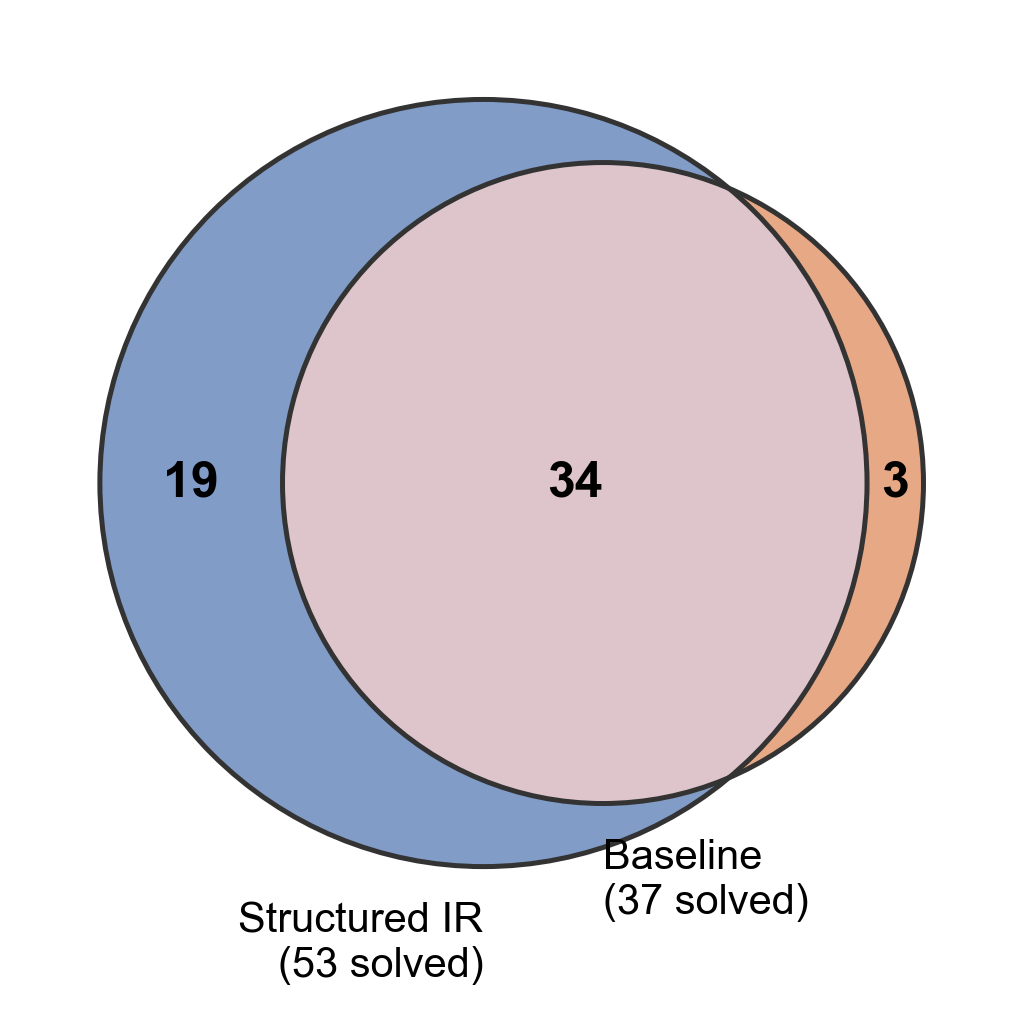
\includegraphics[width=0.5\linewidth]{venn_simple.png}
    \caption{Venn diagram detailing the overlap of solved problems}
    \label{fig:venn_breakdown}
\end{figure}
\begin{itemize}
    \item \textbf{Intersection (Both Solved):} 34 theorems were solved by both methods.
    \item \textbf{Structured-Only Wins:} Our method solved \textbf{19} theorems that the baseline failed to solve.
    \item \textbf{Baseline-Only Wins:} The baseline solved only \textbf{3} theorems that our method missed.
\end{itemize}

This strong asymmetry (19 wins vs. 3 losses) indicates that structural guidance does not merely trade off one type of reasoning for another; rather, it strictly dominates the unguided approach in this resource-constrained regime. Using a paired McNemar test on per-theorem outcomes, the improvement is statistically significant ($p < 0.001$, two-tailed).

\subsection{Failure Mode Analysis}
We analyzed the compilation logs for the failed attempts, classifying errors by the first diagnostic returned by Lean's JSON output. Table~\ref{tab:errors} summarizes the distribution of error types across all failed attempts.

\begin{table}[h]
\centering
\begin{tabular}{lcc}
\hline
\textbf{Error Type} & \textbf{Baseline (\%)} & \textbf{Structured IR (\%)} \\
\hline
unsolved\_goals & 32.9 & 30.4 \\
syntax\_error & 30.0 & 29.3 \\
unknown\_identifier & 18.4 & 19.9 \\
other & 14.5 & 15.2 \\
typeclass\_error & 2.4 & 2.6 \\
type\_error & 1.9 & 2.1 \\
\hline
\end{tabular}
\caption{Distribution of first-failure error types across failed attempts (Baseline: 207 failures, Structured IR: 191 failures). The error distributions are similar, suggesting the Structured IR's gains come from successfully completing proofs that would otherwise fail, rather than from shifting the failure mode.}
\label{tab:errors}
\end{table}

Notably, the error distributions between methods are qualitatively similar. This suggests that the Structured IR's performance gains do not come primarily from avoiding specific error types, but rather from guiding the model toward successful proof completions more often. By enforcing a valid tactic skeleton at the start of generation, the model may avoid early missteps that cascade into failures---the skeleton provides a ``warm start" that increases the probability of reaching a valid proof, even though failed attempts still exhibit similar error patterns. The 16 additional theorems solved (53 vs.\ 37) represent cases where the skeleton-guided generation happened to align with the correct proof strategy.


\section{Discussion}
Our findings challenge the assumption that ``more scale" is the only path to better theorem proving. By simply enforcing valid structural priors---specifically, valid tactic skeletons---we achieved a \textbf{43\% relative improvement} in pass rate.

Interestingly, our error analysis (Table~\ref{tab:errors}) shows that the failure mode distribution remains similar between methods. This suggests that the Structured IR's gains come not from systematically avoiding particular error types, but from increasing the hit rate on successful proofs. The skeleton acts as a ``seed" that, when aligned with the correct proof strategy, guides the model to completion; when misaligned, it fails in similar ways to unguided sampling. The key advantage is that by cycling through diverse skeletons, we increase the probability that at least one attempt aligns with a viable proof strategy.

Furthermore, under the strict constraint ($k=16$, 1024 tokens), our method strictly dominates the unguided baseline (19 unique solves vs.\ 3). This suggests that for resource-constrained applications---where massive tree search is infeasible---structural guidance via a fixed prompt schedule is a more efficient lever than pure stochastic sampling.

\section{Limitations \& Future Work}
The primary limitation of this study is the strict computational budget. Due to resource constraints, we limited generation to 1024 tokens, which likely truncated valid proofs that required verbose Lean states. While this serves as a rigorous test of low-latency performance, it prevents a direct comparison with state-of-the-art leaderboards that utilize extended context windows and massive sampling ($k > 1000$). Additionally, we report results from a single run with one seed and one decoding configuration; we did not sweep multiple random seeds or decoding settings, so run-to-run variability remains unmeasured.

Future work will explore two directions:
\begin{itemize}
    \item \textbf{Scaling the IR:} Investigating whether this structural guidance continues to provide gains when scaled to larger budgets (e.g., $k=128$) or stronger base models.
    \item \textbf{Dynamic Skeletons:} Currently, our tactic skeletons are fixed. A learned ``skeleton retriever" that dynamically predicts the best structure for a given theorem could further refine the query generation process.
\end{itemize}

\appendix

\section{Prompts and Skeleton List}
\label{app:prompts}

\subsection{Prompt Template}
For DeepSeek-Prover-V1.5-RL, we use completion-style prompting (no chat template). The prompt format is:

\begin{verbatim}
/- Lean 4 with Mathlib4 -/
import Mathlib

open BigOperators Real Nat Topology

<theorem statement>
:= by
  <tactic skeleton>
\end{verbatim}

The model then generates the proof completion after the skeleton prefix.

\subsection{Tactic Skeletons}
We use the following 15 tactic skeletons, cycled through for each theorem. For $k=16$, the 16th attempt reuses skeleton 1 (empty) paired with a generic goal hint.

\begin{enumerate}
\item (empty) --- no prefix
\item \texttt{simp}
\item \texttt{intro}
\item \texttt{intros}
\item \texttt{constructor}
\item \texttt{refine ?\_}
\item \texttt{refine \ensuremath{\langle}?\_,\,?\_\ensuremath{\rangle}}
\item \texttt{aesop}
\item \texttt{norm\_num}
\item \texttt{linarith}
\item \texttt{nlinarith}
\item \texttt{ring}
\item \texttt{ring\_nf}
\item \texttt{simp} $\to$ \texttt{try aesop}
\item \texttt{simp} $\to$ \texttt{try nlinarith}
\end{enumerate}

\noindent The 16th attempt uses skeleton 1 with the hint: ``Start by simplifying the goal and hypotheses using \texttt{simp}.''

\section{Environment and Evaluation Harness}
\label{app:env}

\subsection{Lean Environment}
\begin{itemize}
\item \textbf{Lean version:} Lean 4 v4.27.0-rc1
\item \textbf{Mathlib commit:} \texttt{3c327186024184e988ebbcae1b7d7795eaacdee3}
\item \textbf{Verification command:} \texttt{lake env lean --json <file.lean>}
\end{itemize}

\subsection{Model Configuration}
\begin{itemize}
\item \textbf{Model:} \texttt{deepseek-ai/DeepSeek-Prover-V1.5-RL}
\item \textbf{Temperature:} 0.6 (for pass@$k$ sampling)
\item \textbf{Top-$p$:} 0.95
\item \textbf{Max tokens:} 1024
\item \textbf{Per-attempt timeout:} 60 seconds
\end{itemize}

\subsection{Pass Criteria}
A theorem is considered solved if:
\begin{enumerate}
\item Lean returns exit code 0 (successful compilation)
\item The generated proof does not contain \texttt{sorry}
\end{enumerate}

\bibliographystyle{acm}
\bibliography{refs}

\end{document}